% Documentclass options:
%    10pt, 11pt, 12pt  -- set type size
%    draft             -- single space, mark overfull hboxes on paper
%    final             -- double space, don't mark overfull hboxes on paper
%    oneside           -- format for one-sided printing
%    twoside           -- format for two-sided printing
% Defaults are 11pt,final,oneside.  Keep these, please.
\documentclass[11pt]{ucscthesisbs}
\bibliographystyle{apalike2}
\usepackage{natbib}
\usepackage{graphicx,epsf}% Include figure files


% The following declaration is for citations and bibliographies consistent with
% Astrophysical Journal specifications.  It may be left out or replaced with
% another bibliography/citation style.  See also the "\bibliographystyle"
% command later in this file.
%\usepackage{apj}

\usepackage{xcolor}
\usepackage{pagecolor}
\usepackage{lipsum}  

% \pagecolor{darkgray}
% \color{white}

\pagecolor{white}
\color{black}


\begin{document}

% Declarations for Front Matter

\title{Condensation-inhibited convection and thermal evolution of uranus and neptune}
\author{Robert Schroder}
\degreeyear{2020}
\degreemonth{November}
\degree{BACHELOR OF SCIENCE}
\field{ASTROPHYSICS}%
% Declare up to five committee members.  The text will be reproduced directly
% on the signature page.  Though the chair is a committee member, leave
% him/her out of the \committeemember declarations.  Make sure \numberofmembers
% agrees with the number of committee members declared INCLUDING the chair.
% If it is wrong, you will get extra or missing lines on the signature page.
%
\chair{Bruce Schumm}
\thesisadvisor{Christopher Mankovich}
\technicaladvisor{Jonathan Fortney}
\numberofmembers{3}




\campus{Santa Cruz}

\maketitle
\copyrightpage

\begin{frontmatter}

\begin{abstract}
This will be the last section written, once we have finished our analysis.
\end{abstract}

\tableofcontents
%
% The most recent (10/95) guidelines make absolutely no mention of the list
% of figures and list of tables.  Are they necessary?  If not, comment the
% next two lines out.
%
\listoffigures
\listoftables

\begin{dedication}
\null\vfil
{\large
\begin{center}
To Who,\\\vspace{12pt}
the owl
\end{center}}
\vfil\null
\end{dedication}

\begin{acknowledgements}
I'd like to thank my attorney, Bob Loblaw
\end{acknowledgements}


\end{frontmatter}

%\part{First Part}

\chapter{Introduction}
When planets form from their protoplanetary disk, they heat due to the release of gravitational potential, AMONG OTHER THINGS, energy as they collapse upon themselves. The collapse eventually stops as they reach hydrostatic equilibrium, and they finally begin to cool as they release this latent heat of formation through the top of their atmosphere. There are deviations from this evolutionary track, as when terrestrial planets undergo a greenhouse effect, or warm due to the formation of a secondary atmosphere created by outgassing of cooling molten material. Planets may migrate closer to their parent star, increasing the amount of stellar radiation absorbed by the planet's atmosphere. In our solar system, the giant planets are far from the Sun and primarily of solar composition. We are not concerned with those warming scenarios here. In this paper, we confine ourselves to the thermal evolution of the planet Uranus. Uranus is closer to the Sun than its neighbor, Neptune, with which it shares similarities in mass and chemical composition. Strikingly, Uranus is cooler than its more distant counterpart. Much work has been done with model atmospheres. These models assume a thoroughly convective atmosphere along a dry adiabat and have been consistently at odds with observation of Uranus. They do not predict the under-luminous Uranus that we now observe. In this paper, we explore the impact of condensation-inhibited convection on the planet's thermal evolution to see if it offers a possible explanation for current observations. In section 1.1, we review prior work done on model atmospheres of solar system giant planets. In section 1.2, we review prior work done on the formation of water condensation zones in these hydrogen rich atmospheres. In chapter 2, we describe our model and present our results. In chapter 3, we discuss the ramifications of condensation inhibited convection for the thermal evolution of Uranus. Finally, in chapter 4, we summarize our findings.\citep{friedson_2017} \citep{leconte_2017} \citep{pollack_1977}\citep{fortney_2011} \citep{graboske_1975} \citep{guillot_2019} \citep{guillot_1995}

test

\section{Model Uranus and Neptune with Dry Convection}\label{model_atmosphere_background}

Will review current understanding of solar system giant planet thermal evolution here, referencing work done by Fortney, et al., and others. Not sure how far back I want to go here, but will probably mention when, and by who, thermal evolution modeling began, and then quickly get into the thermal evolution background from fortney papers.

\begin{figure}[ht!]
 \centerline{
  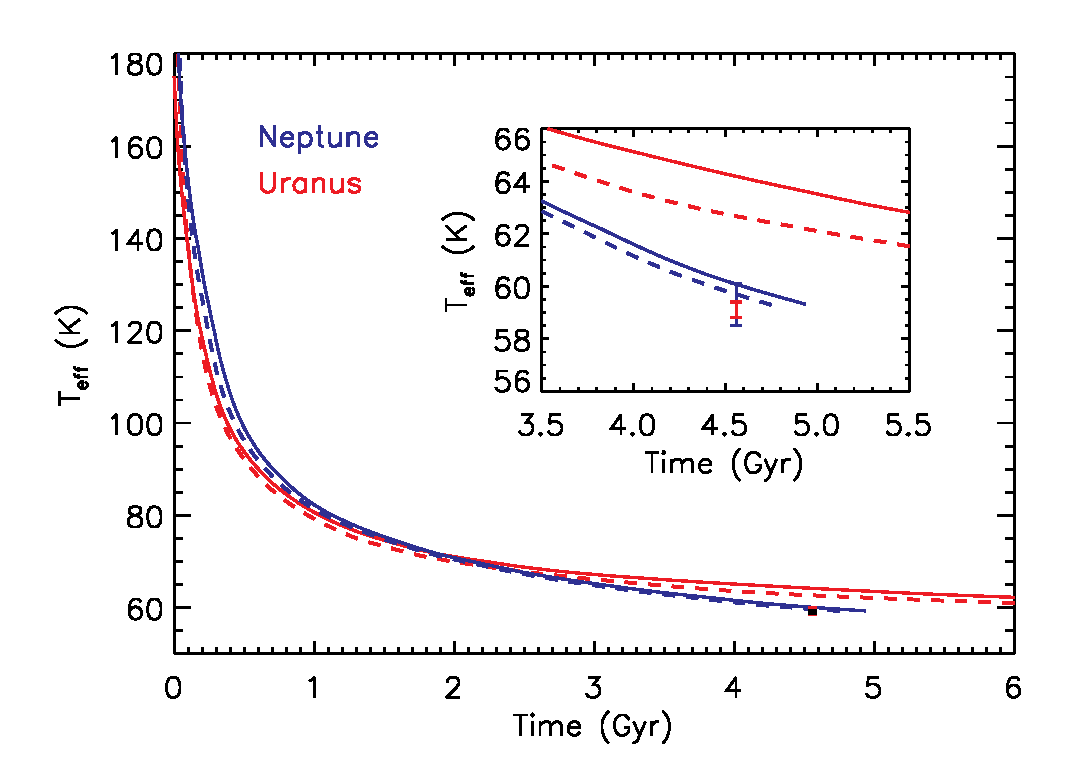
\includegraphics[width=4.0in]{figures/f10.eps}
 }
\caption[This is just a placeholder for our own plot]
{Thermal evolution of Uranus and Neptune 
}

\label{fig:discretescan}
\end{figure}


\section{Condensation-inhibited Convection}\label{condensation_background}

This section will contain theory and results surrounding condensation in hydrogen rich atmospheres, citing LeConte, Friedson, others.


\chapter{Model Uranus and Neptune with Condensation-inhibited Convection}

\section{Numerical Model}

\section{Results}

\begin{figure}[ht!]
 \centerline{
  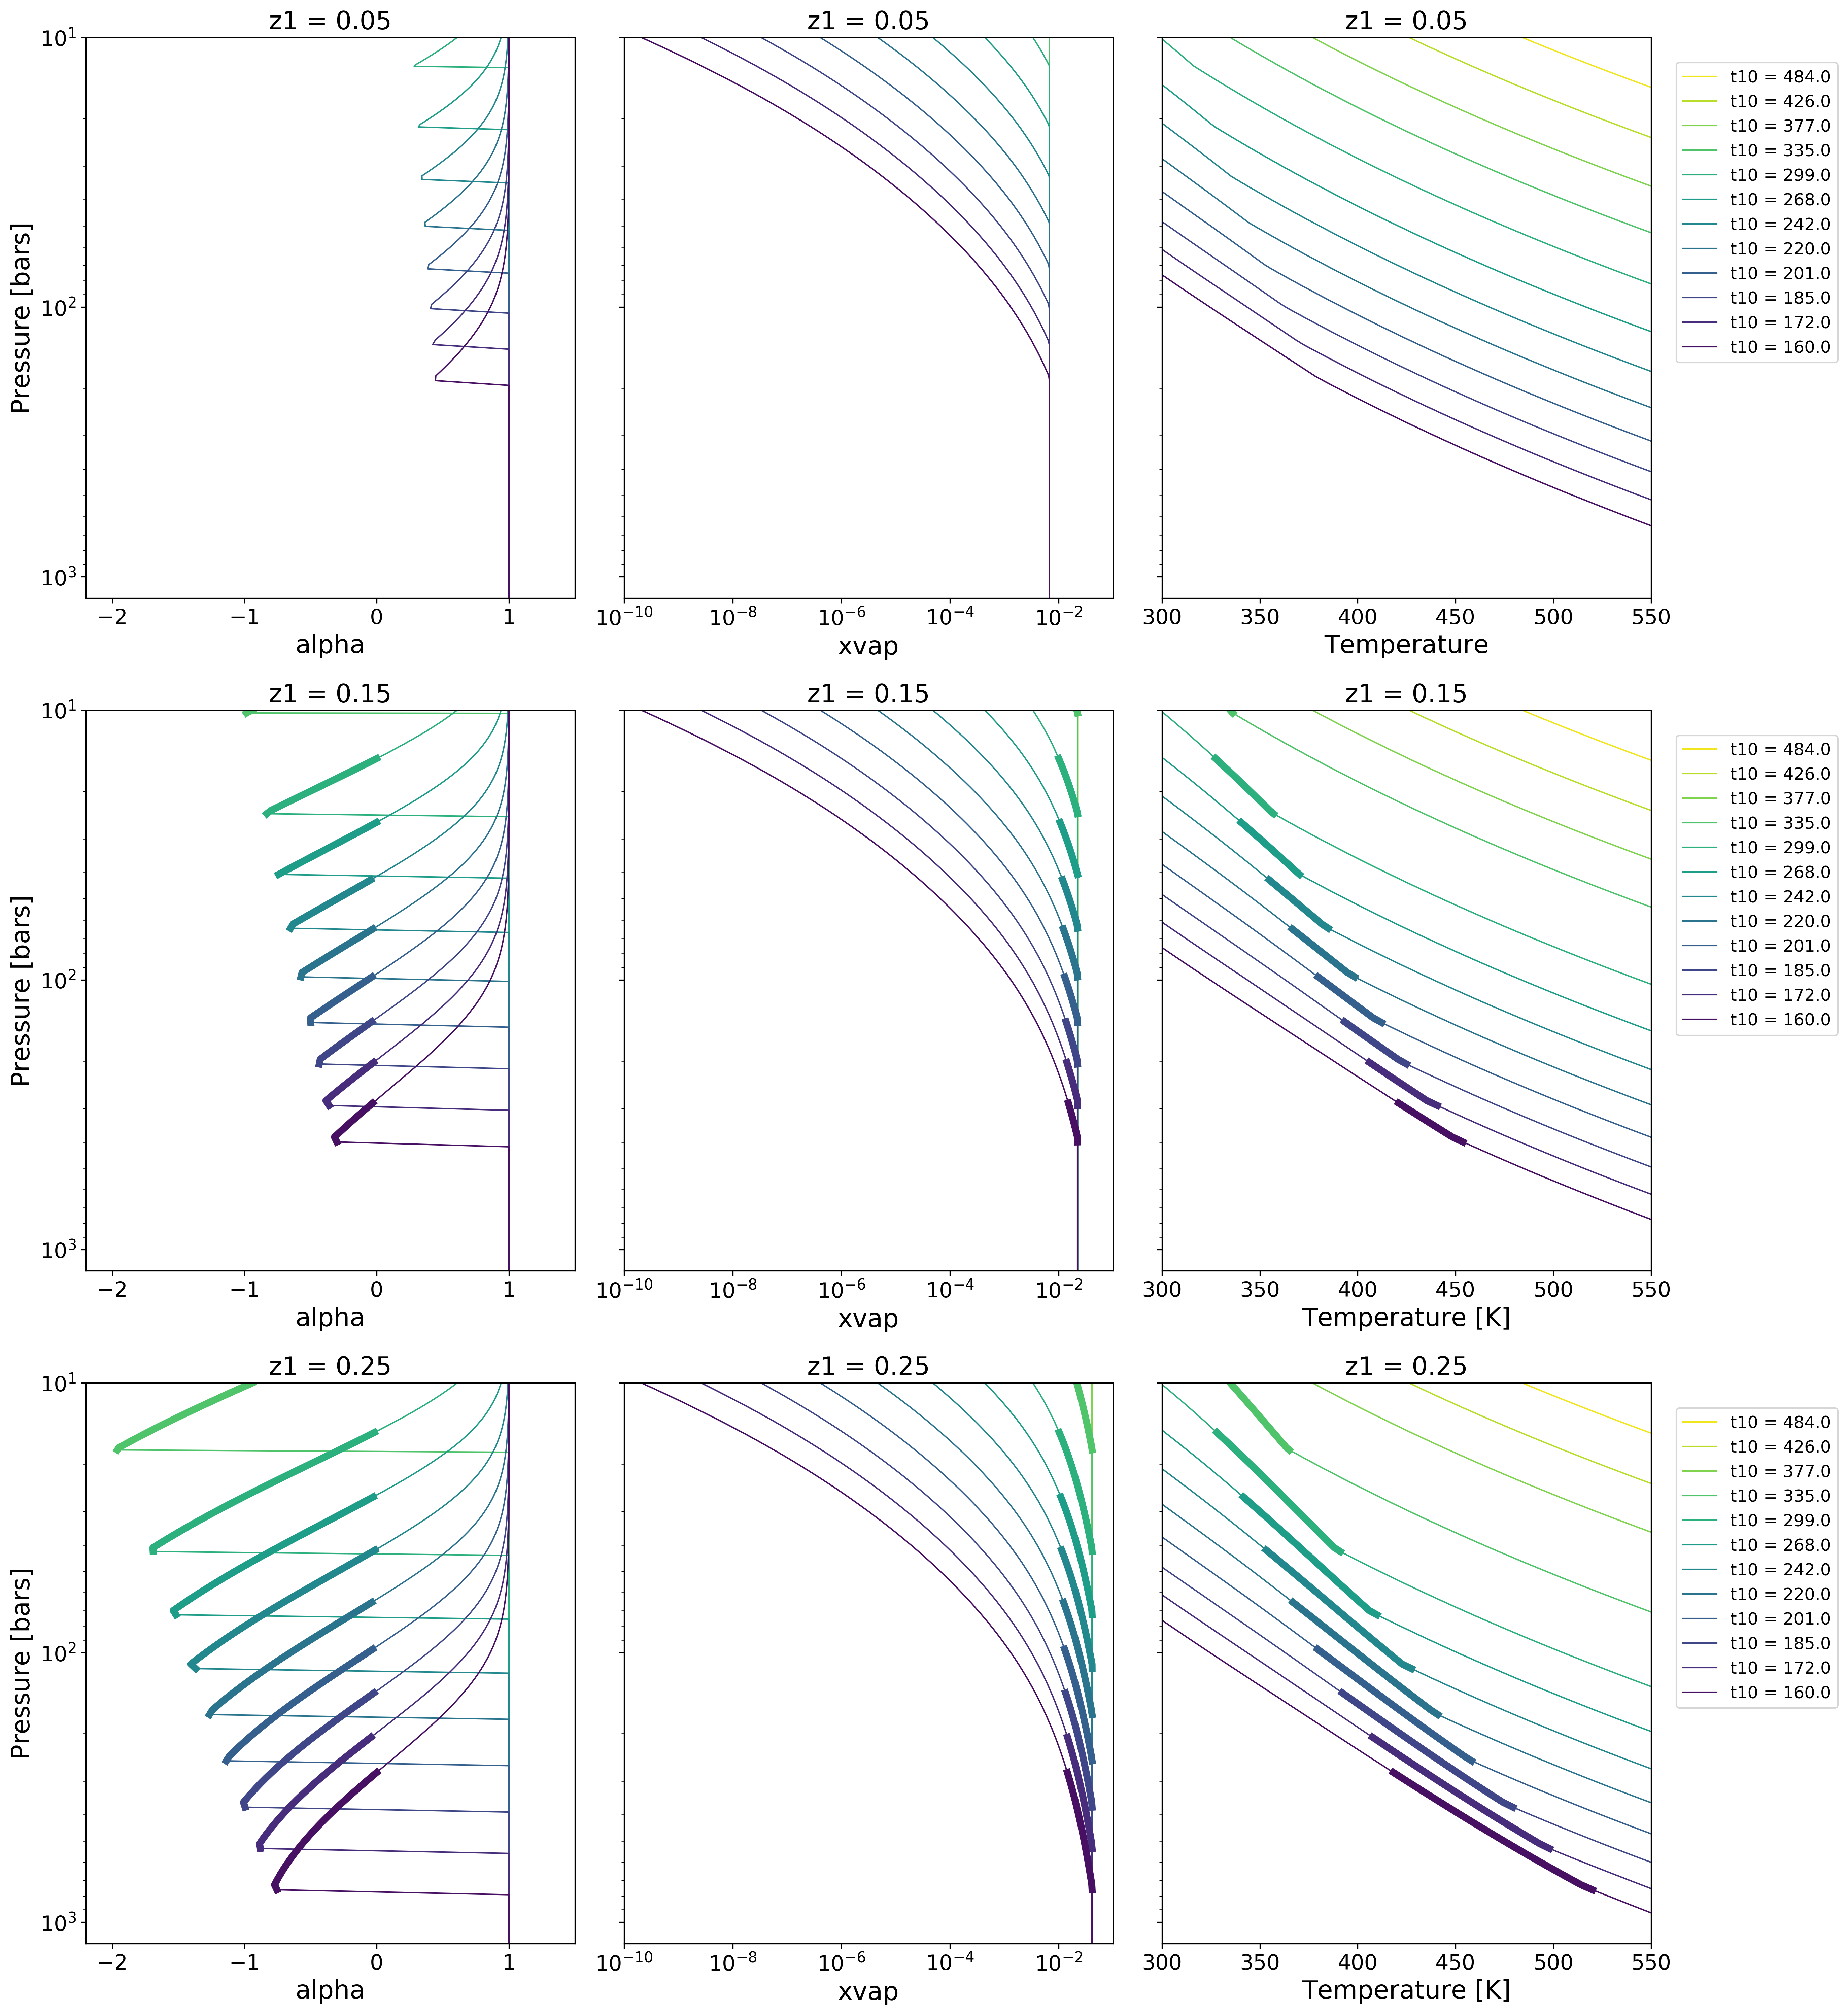
\includegraphics[width=7.0in]{figures/convection_inhibited_2.png}
 }
\caption[Inhibition of convection on Uranus]
{Need to add description here }
\label{fig:uranus}
\end{figure}
\begin{figure}[ht!]
 \centerline{
  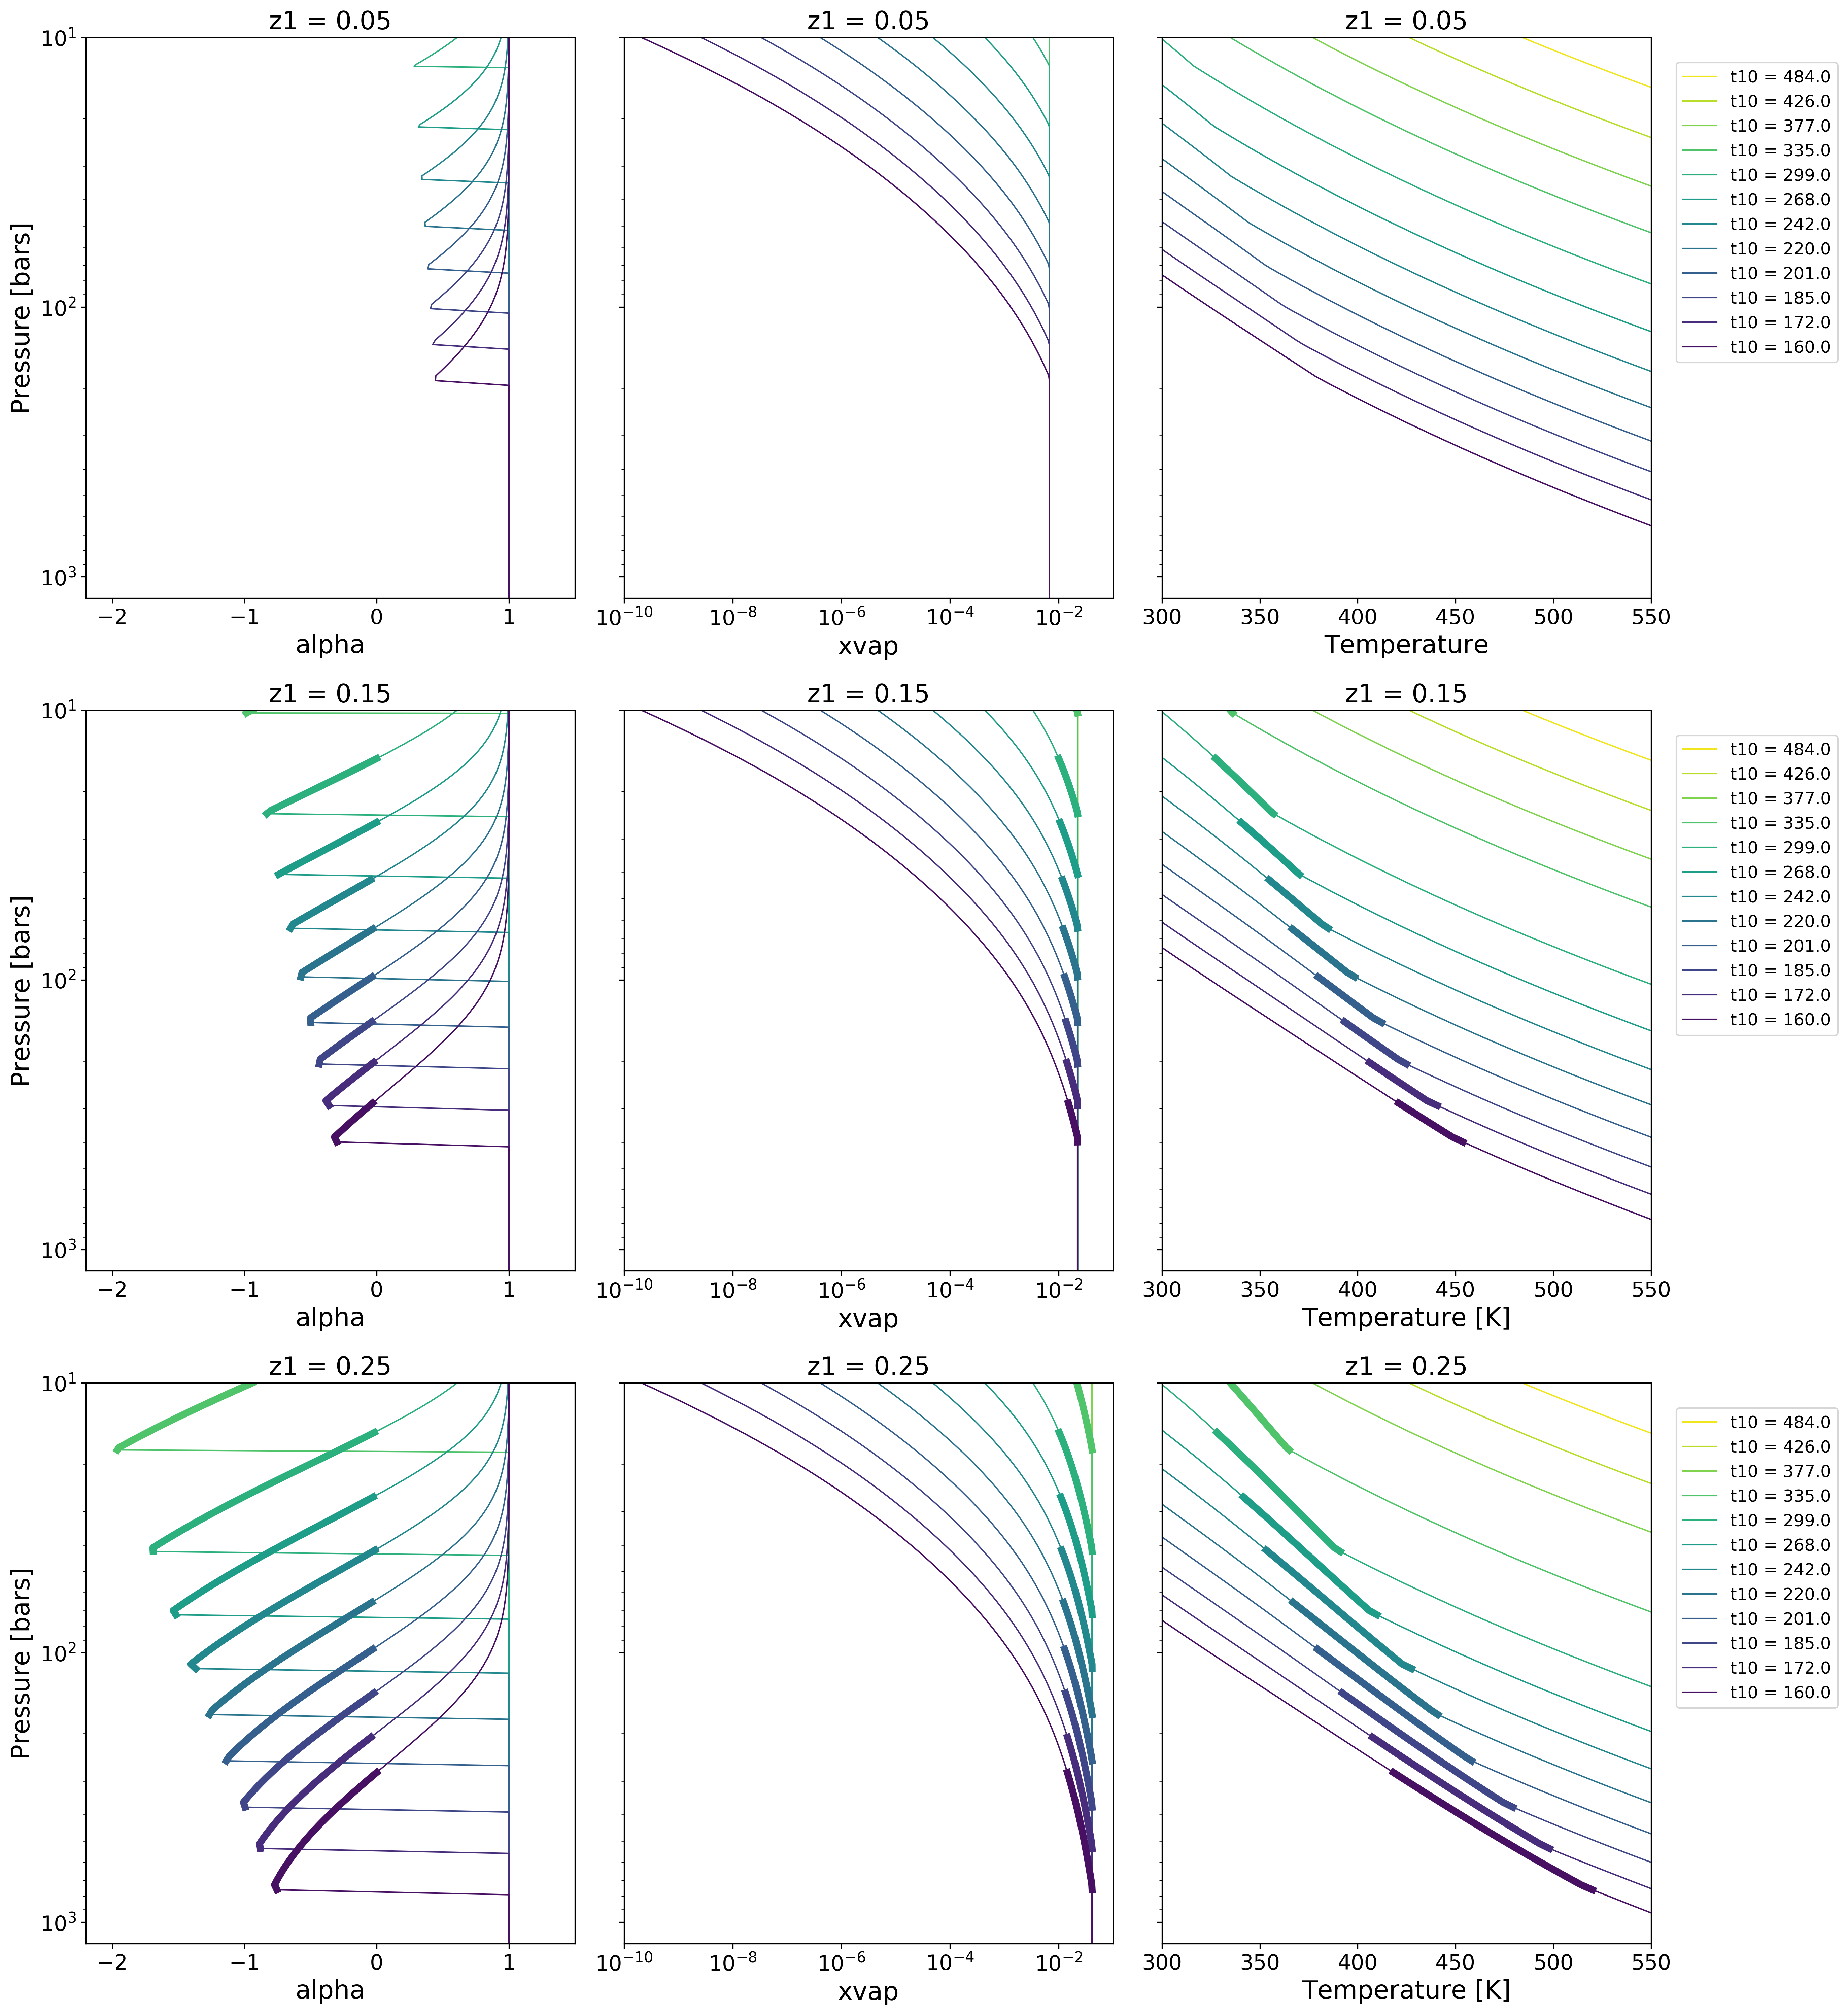
\includegraphics[width=7.0in]{figures/convection_inhibited_2.png}
 }
\caption[Inhibition of convection on Neptune]
{Need to add description here }
\label{fig:neptune}
\end{figure}


\chapter{Discussion and Conclusions}





\appendix
\chapter{Some Ancillary Stuff}

Ancillary material should be put in appendices.  The guidelines are not
clear whether bibliography comes before or after the appendices, but they
\emph{suggest} appendices come first.
Ancillary material should be put in appendices.  The guidelines are not
clear whether bibliography comes before or after the appendices, but they
\emph{suggest} appendices come first.
Ancillary material should be put in appendices.  The guidelines are not
clear whether bibliography comes before or after the appendices, but they
\emph{suggest} appendices come first.
Ancillary material should be put in appendices.  The guidelines are not
clear whether bibliography comes before or after the appendices, but they
\emph{suggest} appendices come first.



\bibliography{wcz_bib}


\end{document}
